\documentclass[oneside]{VUMIFPSkursinis}
\usepackage{algorithmicx}
\usepackage{algorithm}
\usepackage{algpseudocode}
\usepackage{amsfonts}
\usepackage{amsmath}
\usepackage{bm}
\usepackage{caption}
\usepackage{color}
\usepackage{float}
\usepackage{graphicx}
\usepackage{listings}
\usepackage{subfig}
\usepackage{wrapfig}

\university{Vilniaus universitetas}
\faculty{Matematikos ir informatikos fakultetas}
\department{Programų sistemų katedra}
\papertype{Laboratorinis darbas I}
\title{Automatinė ūkio valdymo sistema}
\titleineng{Automatic farm management system}
\status{2 kurso 3 grupės studentai}
\author{Matas Savickis}
\secondauthor{Justas Tvarijonas}   % Pridėti antrą autorių
\thirdauthor{Greta Pyrantaitė}   % Pridėti trečią autorių
\fourthauthor{Rytautas Kvasinskas}   % Pridėti ketvirtą autorių
\supervisor{Karolis Petrauskas, Doc., Dr.}
\date{Vilnius – \the\year}

% Nustatymai
% \setmainfont{Palemonas}   % Pakeisti teksto šriftą į Palemonas (turi būti įdiegtas sistemoje)
\bibliography{bibliografija}

\begin{document}
\maketitle

\tableofcontents



\sectionnonum{Įvadas}
Automatinė ūkio valdymo sistema(toliau Auto ūkis) - yra programa leidžianti ūkininkui valdyti jo ūki skaitmeniniu būdu. Auto ūkis  leidžia stebėti kiekvieno individualaus gyvūno bioparametrus(kraujo spaudima, svorį, sveikatą), ūkio technikos judėjimą po žemės plota, gyvūnų registracija. Taip pat sistema vartotojui leidžia sekti dirvos parameturs(drėgmę, pH lygi),  oro prognozes ir aplinkinių teritorijų gyvūnų ligų paplitimą. Auto ūkis padeda ir su verslo valdymu, nesunkiai galima samdyti darbuotojus, atlikti buhalterinę apyskaita, stebėti rinkos kainas ir skaičiuoti bei numatyti galimą pelną. Iškilus nelaimės per Auto ūkio sistemą galima greitai iškviesti greitąją pagalba, policiją, gaisrinę ar saugos tarnybą. Orai prognozės yra paimtos iš www.gismeteo.lt. Pagrindinė sistemos inovacija yra tai, kad kai sistema yra pilnai įdiegta darbuotojų skaičius palaikyti ūki tampa minimalus. Ūkio technika būtų valdoma automatiškai todėl vairuotojų ir derliaus nurikėjų nereiktų. Gyvūnų sekimas yra įgyvendinamas microkontrolerio Arduino pagalba. Kadangi šis kontroleris ledidelis ir lengvai pritaikomas visiokio pobūdžio darbams ji kartu su WiFi moduliu sistema naudoja gauti gyvųno lokacija per Google maps. Taip pasiklydę ar pavogti gyvųnai būtų greitai gražinami surandami ir gražinami. Žemės laistymas, tręšimas taip pat būtų automatizuotas, parametrai gaunami per Arduino detektorius, kurie pagal pasikeitusia dirvos kompozicija nusprendžia ko trūksta žemei ir aktyvuoja laistymo ir tręšimo sistemas. Auto ūkio sistema yra parašyta JAVA kalba kas leidžia programą paleisti ant betkurios operacinės sistemos. Ateityje numatoma galimybė programą perkelti į išmaniuosius telefonus. Sistema buvo projektuojama pasitelkiant www.planttext.com ir www.draw.io funkcionalumą.

\sectionnonum{Žodymas}
\begin{itemize}
	\item Klasės:
		\begin{itemize}
			\item AutoŪkis - pagrindinė(main) programos klasė. Ši klasė piešia grafinę vartotojo sąsaja ir laiko savyje kitų klasių objektus kurių informacija reikalinga piešimui
			\item Map - teritorijos piešimui skirta klasė.
			\item ŽemėsTeritorija - apskaičiuoja tam tikros teritorijos plotą.
 			\item Gyvūnas - klasė skirta gyvūno rodmenims ir metodams saugoti
			\item AriamasLaukas - laiko savyje reikšmes apibūdinančias unikalų lauką ir metodus susijusius su lauko darbu.
			\item Ganykla - laiko parametrus ir metodus darbui su ganyklomis kurios yra žemės plote.
			\item ŪkinisPastatas - saugo ūkinius 
			\item ŪkioTechnika - laiko ūkio technikos charakteristikos reikšmes. Apskaičiuoja technikos judėjimo greitį.
			\item Žemės parametrai - saugo įvairius žemės parametrus(drėgmė, ph...).
			\item Orai - klasė skirta pasiimti orų prognozes iš www.gismeteo.lt kurių paprašo vartotojas.
			\item Žemės detektorius - klasė skirta bendrauti su žemės detektoriumi

		\end{itemize}
	\item Bendri terminai:
		\begin{itemize}
			\item Žemės plotas - vieta kurią valdo ir gali stebėti vartotojas(ūkininkas) 
		\end{itemize}
\end{itemize}

\section{Sukurtos sistemos aprašymas(v1.0)}

\subsection{Loginis pjūvis}
	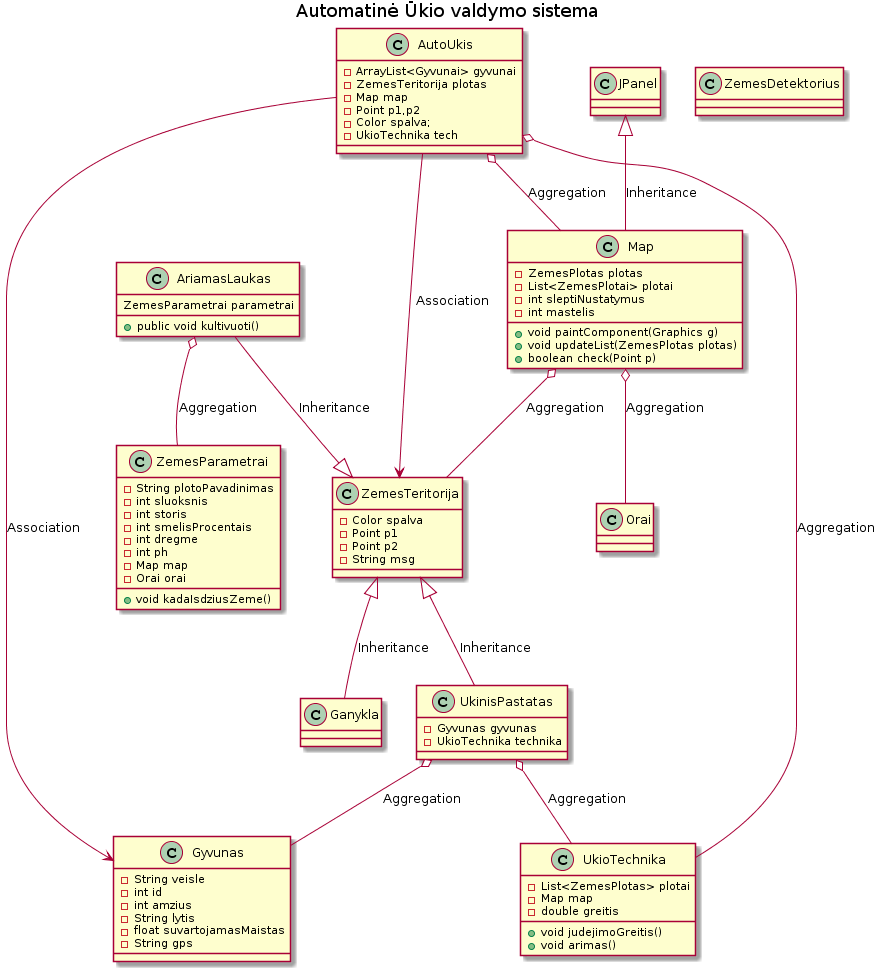
\includegraphics[width=\textwidth,height=\textheight,keepaspectratio]{uml.png}	
	Suprogramavę šabloninį programos programos karkasą nubraižėme UML diagramą pasinaudoja minėta PlantText programą. 
	\begin{itemize}
		\item Dizainas: 
		\begin{itemize}
			\item Programos pagrindas yra AutoUkis.form klasė kuri pasiima duomenis iš kitų klasių. O duomenis įveda patys vartotojai. Rašant kodą stengėmės prisilaikyti objektinio programavimo principų. GUI piešimas ir pasirinkimas vyko AutoUkis klasėje kurį pasiima duomenis iš kitų klasių. Daugumos objektų kūrimas ir laikymas taip pat yra šioje klasėje. Visos kitos klasės turėjo savo atskiras paskirtis(Gyvūnas - saugojo duomenis, Map - piešė žemėlapį). Kai kurios klasės(pvz. : ZemesDetektorius) buvo sukurtos dėl dizaino tolimesnio jų panaudojimo, bet nebuvo niekur pritaikytos.
		\end{itemize}
		\item Funkcionalumas:
		\begin{itemize}
		\item Viso užsibrėžto programos funkcionalumo įgyvendinti nepavyko. Kai kurios klasės buvo sukurtos ateityje planuojamoms funkcijoms. Programa kol kas veikia tik ant kompiuterio ir vienintelis jos bendravimas su internetu yra per Orai klasę. Yra funkcija surašyti gyvūnus ir duomenis apie juos ir žymėti bei atlikti primityvią žemės kategorizaciją.
		\end{itemize}	
	\end{itemize}
 
\subsection{Kūrimo pjūvis}
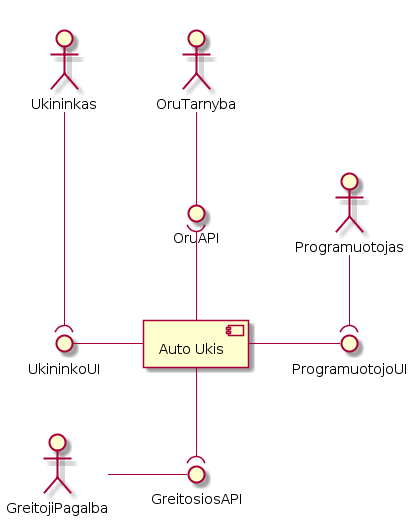
\includegraphics{l0.png}	
	\pagebreak
	\begin{itemize}
		\item Dizainas: 
		\begin{itemize}
			\item Pradėjus rašyti programą nepagalvojome apie kūrimo pjūvį ir kaip teisingiau būtų pradėti viską. Žiūrint dabar visa programa buvo pradėta kurti pagal Bottom -> Up principą. Iš pradžių apsirašėme daugybe mažų klasių ir paskui jas bandėme apjungti į didesnę sistemą. Kai kurios klasės liko nepanaudotos. 
		\end{itemize}
		\item L0:
		\begin{itemize}
			\item Šioje diagramoje pavaizdavome sistemos bendravimą su išoriniais agentais tokiais kaip Greitoji pagalba, Ūkininkas ir t.t. . Ši diagrama aiškiai ir paprastai parodo kuriamus ir įgyvendinamus interfeisus. Galbūt būtų galima Greitosios Pagalbos interfeisą išskaidyti į kelis detalesnius interfeisus, bet apskritai didelių problemų nepastebime.

		\end{itemize}
	\end{itemize}
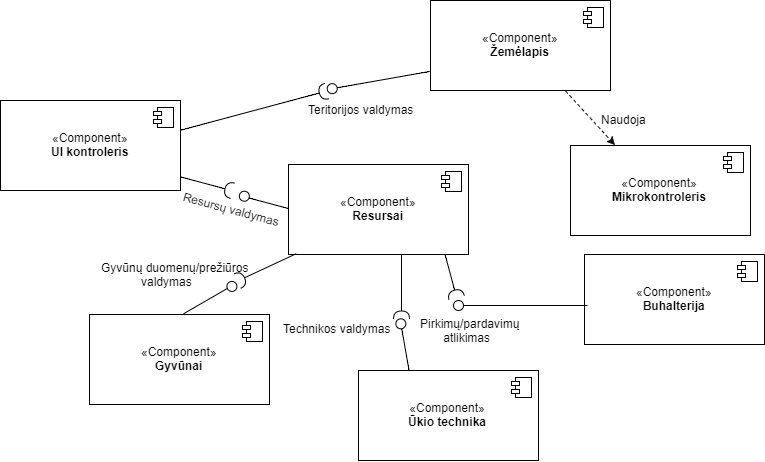
\includegraphics[width=\textwidth,height=\textheight,keepaspectratio]{l1.png}	

\begin{itemize}
	\item L1: Sudėjus komandos idėjas apie tai, kaip turėtų atrodyti L1 diagrama, supratome, kad mūsų sistema neturi normalios struktūros ir gerai nebuvome pagalvoję kaip visi komponentai siesis vieni su kitais, todėl ir diagrama atrodo chaotiška. Trūksta konkretumo kaip turi Admin sietis su kitas komponentais. Programa atsiranda kaip komponentas  kas greičiausiai yra nekorektiška.

\end{itemize}
	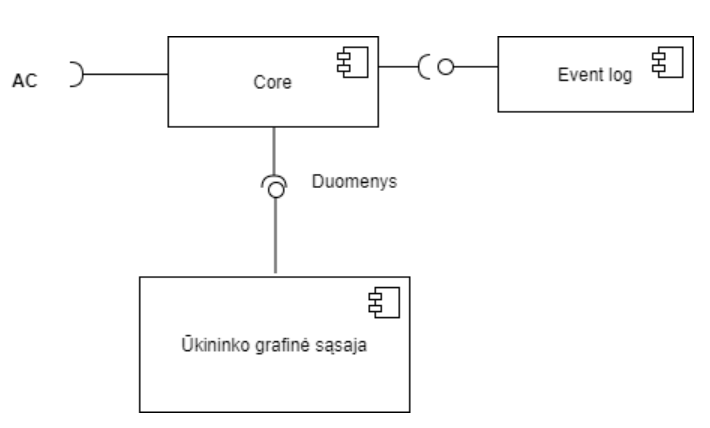
\includegraphics[width=\textwidth,height=\textheight,keepaspectratio]{l2uki.png}

	\begin{itemize}
		\item L2(Ūkininkas): Šioje diagramoje parodyta, kad programos pagrindas kuria suteikia interface’a grafinei vartotojo sąsajai. Paduoti duomenys yra užregistruojami Event Log’e.

	\end{itemize}
	
	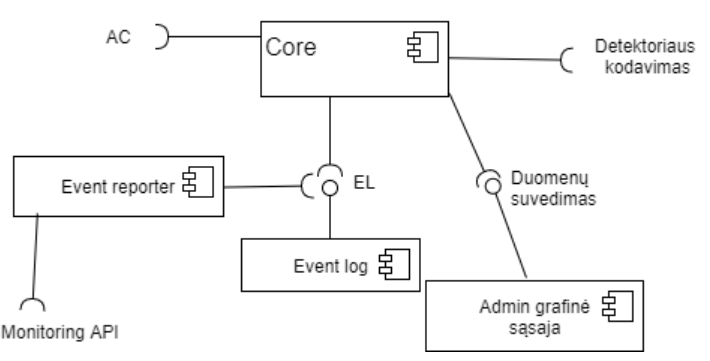
\includegraphics[width=\textwidth,height=\textheight,keepaspectratio]{l2admin.png}
	
	\begin{itemize}
		\item L2(Admin): Šioje diagramoje parodyta,kad programos pagrindas naudoja duomenų suvedimo interface, kurį suteikia admin grafinė sąsaja, bei naudoja Detektoriaus kodavimo interface. Visus įvykius įrašo į event log

	\end{itemize}

		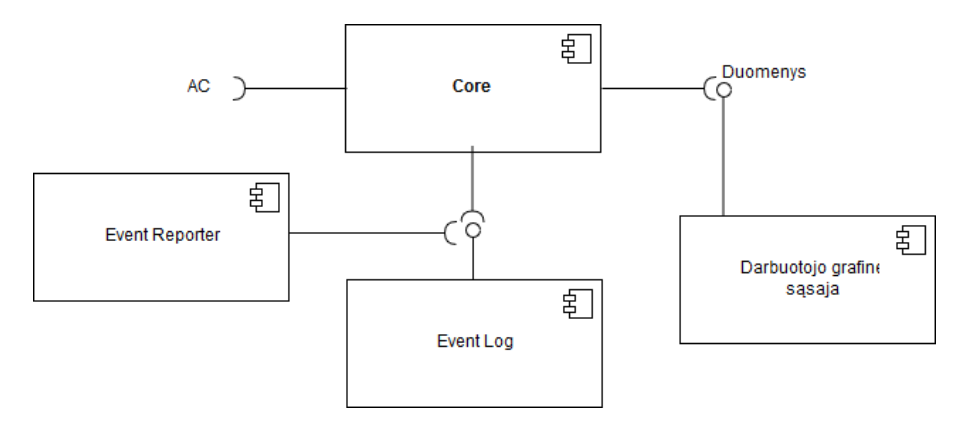
\includegraphics[width=\textwidth,height=\textheight,keepaspectratio]{l2darb.png}

\begin{itemize}
		\item L2(Darbuotojas):Šioje diagramoje parodyta, kad programos pagrindas  grafinę sąsają ir perduoda duomenis į event log’ą. 

	\end{itemize}

		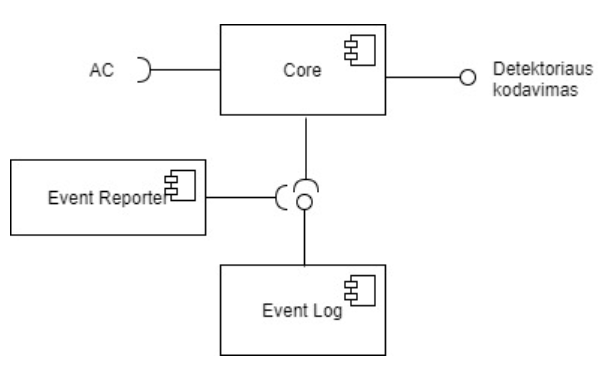
\includegraphics[width=\textwidth,height=\textheight,keepaspectratio]{l2det.png}

\begin{itemize}
		\item L2(Detektorius): ši diagrama vaizduoja detektoriaus išvedamus duomenis. Įvykiai įrašomi Event Log’e.


	\end{itemize}
\pagebreak
		

	

\subsection{Proceso pjūvis}
\subsection{Fizinis pjūvis}

\section{Perprojektuotos sistemos aprašymas(To-Be, v2.0)}
\subsection{Loginis pjūvis}
\subsection{Kūrimo pjūvis}
\subsection{Proceso pjūvis}
\subsection{Fizinis pjūvis}


\sectionnonum{Rezultatai ir išvados}












\end{document}
